
\section{CS6000 Computer Science Research\\ {\sc Week 5 Git Assignment}} 

\begin{center}
    Marwan Alharbi
\end{center}


\subsection{About}
This Fall 2023 I just joined UCCS as PhD student (Fig. \ref{img:alharbi:profile}). It is my first semester in 
this program. Prof. Sudhanshu Semwal is my academic advisor.

My research interests are in Machine Learning, Computer Graphics, and Programming 
Languages. My goal in this course is to learn research fundamentals. The correct 
way to choose state of the art research paper in a selected area. Techniques 
of writing a scientific paper that benefit the world and help me in the future as 
well. Increase my ability to read several research papers in a short time. Learn 
more about how get reader to enjoing reading my research stories.

\begin{figure}[h]
    \centerline{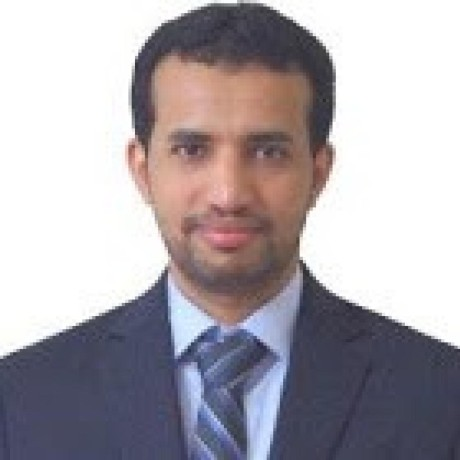
\includegraphics[width=0.3\textwidth]{images/alharbi-f23-profile.jpg}}
    \caption{Marwan's profile photo \label{img:alharbi:profile}} 
\end{figure}

\subsection{Related Research Code}
One of the research studies aligned with my research interests discusses a recommended 
method for improving rendering speed by integrating intermediate deep learning stages 
within the pipeline. The implementation necessitates the utilization of various Python
libraries enabling the execution of specific code segments on a GPU. Testing this 
implementation requires the presence of an NVIDIA GPU.

You may read more about that code on the authors' (Mark Harris and Sudhanshu Semwal) GitHub repository (\textit{checked by: Sep. 2023}):

\url{https://github.com/wharris2-uccs/adlgp}

\subsection{Ask Marwan}

\begin{enumerate}[label={Question \arabic*.}]
    \item First question \dots
    \item Second question \dots
\end{enumerate}
